\chapter{Синтез линейных непрерывных систем}
\setcounter{section}{8} %TODO:Remove
\setcounter{subsection}{2} %TODO:Remove
\setcounter{equation}{23} %TODO:Remove
\setcounter{figure}{7}%TODO:Remove

\subsection{Идентификационное каноническое представление системы с одним (скалярным) выходом}
С помощью рассуждений, аналогичных проведённым в п.3.8.1, можно получить следующие результаты.

Если пара матриц    полностью наблюдаема,  то  в   пространстве состояний  Х  всегда существует базис, в котором пара ${A,C}$  имеет идентификационное каноническое представление (ИКП):
\begin{equation}
	A_I = 
	\begin{bmatrix}
	    0 & 0 & \dots & 0 & 0 & -\alpha_n \\
	    1 & 0 & \dots & 0 & 0 & -\alpha_{n-1} \\
	    0 & 1 & \dots & 0 & 0 & -\alpha_{n-2} \\
	    \dots & \dots & \dots & \dots & \dots & \dots \\
	    0 & 0 & \dots & 0 & 0 & -\alpha_3 \\
	    0 & 0 & \dots & 1 & 0 & -\alpha_2 \\
	    0 & 0 & \dots & 0 & 1 & -\alpha_1
	\end{bmatrix}
\end{equation}

\begin{equation}
	C_I = 
	\begin{bmatrix}
	    0 & 0 & \dots & 0 & 0 & 1
	\end{bmatrix}
\end{equation}

Отметим, что

\begin{equation}
	A_I^T = A_U; C_I^T=\vec{b}_U.
\end{equation}

Если   в  некотором  исходном  базисе [$h$] заданы матрицы $A_H, C_H$ и если система полностью наблюдаема, то, для того чтобы вычислить их (матриц) ИКП, достаточно вычислить коэффициенты характеристичес¬кого полинома $\phi_A(\lambda)$ . После этого может быть вычислена матрица преобразования от исходного базиса [$h$] к ИКП в соответствии с (3.7.13):

\begin{equation}
	I_H^{-1}=N_I^{-1}N_H.
\end{equation}

Если известна матрица $B_H$ при векторе управления в исходном базисе, то с учётом (3.6.8)  в базисе ИКП она может быть определена с помощью соотношения

\begin{equation}
	B_I=I_H^{-1}B_H
\end{equation}

\subsection{Передаточная функция и структура для системы в ИКП}
В соответствии с видом матриц $A_I$ и $C_I$ уравнения системы со скалярным входом $u$ и скалярным выходом $y$  имеют вид

\begin{equation}
\begin{cases}
	\dot{x}_{i1} = -\alpha_nx_{in}+b_{i1}u;\\
	\dot{x}_{i2} = x_{i1} - \alpha_{n-1}x_{in}+b_{i2}u;\\
	\dot{x}_{i3} = x_{i2} - \alpha_{n-2}x_{in}+b_{i3}u;\\
	\begin{tabular}{ l l l l l l }
	  \dots & \dots & \dots & \dots & \dots & \dots 
	\end{tabular}
	\dot{x}_{in-1} = x_{in-2} - \alpha_{2}x_{in}+b_{in-1}u;\\
	\dot{x}_{in} = x_{in-1} - \alpha_{1}x_{in}+b_{in}u;\\
\end{cases}
\end{equation}

\begin{equation}
	y = x_{in}
\end{equation}

Этим уравнениям соответствует структурная схема, представленная на рис. 3.8.

\begin{figure}[H]
	\centering
	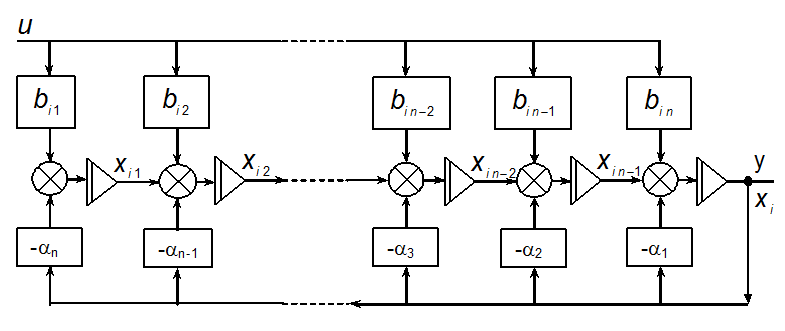
\includegraphics[scale=0.9]{images/Fig3_8}
	\caption{Схема моделирования системы в ИКП}
\end{figure}

В соответствии с этим рисунком передаточная функция системы имеет вид

\begin{multline}
	W_{u,y}(p) = \dfrac{b_{i1}p^{-n}+b_{i2}p^{-(n-1)}+\dots+b_{in-1}p^{-2}+b_{in}p^{-1}}{1+\alpha_1p^{-1}+\alpha_2p^{-2}+\dots+\alpha_np^{-n}} = \\
	\dfrac{b_{i1}+b_{i2}p+\dots+b_{in-1}p^{n-2}+b_{in}p^{n-1}}{p^n+\alpha_1p^{n-1}+\alpha_2p^{n-2}+\dots+\alpha_{n-1}p+\alpha_n}.
\end{multline}

Отметим, что статический передаточный коэффициент

\begin{equation}
	W_{u,y}(0)=\dfrac{b_{i1}}{\alpha_n}
\end{equation}

\newpage

\section{Обратная связь по состоянию, обеспечивающая заданное (желаемое) расположение собственных чисел в замкнутой системе с одним (скалярным) входом}

Даны уравнения полностью управляемого объекта управления в некотором исходном базисе

\begin{gather}
\begin{split}
	&\dot{\vec{x}}_H(t) = A_H\vec{x}_H(t)+\vec{b}_Hu(t);\\
	&y(t)=C_H\vec{x}_H(t),
\end{split}
\end{gather}
каждая координата вектора состояния которого доступна для измерения.
Требуется синтезировать такое управление, которое бы обеспечило требуемое качество отработки внешнего командного сигнала $v(t)$.

Динамические свойства системы управления в основном определяются её собственными числами, то есть нулями характеристического полинома
\begin{equation}
	\phi_A(\lambda) = \prod_{i=1}^{n}(\lambda - \lambda_i)=\lambda^n+\alpha_1\lambda^{n-1}+\dots+\alpha_n.
\end{equation}

Время переходного процесса каждой моды определяется расстоянием до мнимой оси вещественной части; колебательность - соотношением мнимой и вещественной частей соответствующих собственных чисел. Эти зависимости могут быть проанализированы при изучении характеристик типовых звеньев, кроме того, они рассматриваются в обширной учебной литературе по теории автоматического регулиро-вания и управления.

В соответствии со структурной схемой, приведённой на рис. 3.9, сформируем сигнал управления объектом в виде
\begin{equation}
	u(t) = L_H\vec{x}_H(t) + k^vv(t)
\end{equation}
где $L_H$ – некоторая матрица-строка обратной связи:
\begin{equation}
	L_H = [\begin{tabular}{ l l l l }
		  	$l_{h1}$ & $l_{h2}$ & $\dots$ & $l_{hn}$
		  \end{tabular}]
\end{equation}
$k^v$ – коэффициент по командному сигналу.
Тогда уравнение системы примет вид
\begin{equation}
	\dot{\vec{x}}_H(t)=A_H\vec{x}_H(t)+\vec{b}_HL_H\vec{x}_H(t)+\vec{b}_Hk^vv(t),
\end{equation}
или
\begin{equation}
	\dot{\vec{x}}_H(t)=A_H^C\vec{x}_H(t)+\vec{b}_Hk^vv(t),
\end{equation}
где $A_H^C$ - матрица замкнутой системы в исходном базисе:
\begin{equation}
	A_H^C=A_H+\vec{b}_HL_H
\end{equation}

\begin{figure}[H]
	\centering
	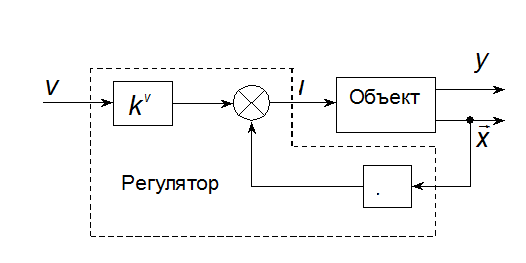
\includegraphics[scale=0.9]{images/Fig3_9}
	\caption{Структурная схема замкнутой системы}
\end{figure}

Поскольку объект полностью управляем, то существует базис [$u$], в котором пара $\{A,\vec{b}\}$ имеет управляемое каноническое представление $\{A_U,\vec{b}_U\}$ . Поэтому перейдём к записи уравнений системы в базисе УКП. В соответствии с (3.4.16) произведём замену 
\begin{equation}
	\vec{x}_H=U_H\vec{x}_U
\end{equation}
Тогда из (3.9.1) получим
\begin{equation}
	U_H\dot{\vec{x}}_U(t)=A_HU_H\vec{x}_U(t)+\vec{b}_Hu(t);
\end{equation}
\begin{equation}
	y(t)=C_HU_H\vec{x}_U.
\end{equation}
Умножив уравнение (3.9.9) слева на $U_H^{-1}$, будем иметь
\begin{gather}
\begin{split}
	&\dot{\vec{x}}_U(t)=A_U\vec{x}_U(t)+\vec{b}_Uu(t);\\
	&y(t) = C_U\vec{x}_U(t),
\end{split}
\end{gather}
где $A_U$ $\vec{b}_U$ и $C_U$ - соответствующие матрицы в УКП.

Используя подстановку (3.9.8), из (3.9.3) получим
\begin{equation}
	u(t)=L_U\vec{x}_U+k^vv(t),
\end{equation}
где матрица обратной связи в базисе УКП
\begin{equation}
	L_U=L_HU_H.
\end{equation}

В результате  уравнение замкнутой системы  в базисе управляемого канонического представле¬ния будет иметь вид
\begin{equation}
	\dot{\vec{x}}_U(t)=A_U^C\vec{x}_U(t)+\vec{b}_U \cdot k^vv(t)
\end{equation}
Здесь $A_U^C$ является сопровождающей матрицей по отношению к характеристическому полиному замкнутой системы
\begin{equation}
	\phi_{A^C}(\lambda) - \prod_{i=1}^{n}(\lambda - \lambda_i^3)=\lambda^n+\gamma_1\lambda^{n-1}+\dots+\gamma_n,
\end{equation}
поэтому она имеет стандартный вид
\begin{equation}
	A_U^C = 
	\begin{bmatrix}
	    0 & 1 & 0 & \dots & 0 \\
	    0 & 0 & 1 & \dots & 0 \\
	    \dots & \dots & \dots & \dots & \dots \\
	    0 & 0 & 0 & \dots & 1 \\
	    -\gamma_n &  -\gamma_{n-1} & -\gamma_{n-2} & \dots & -\gamma_1 \\
	\end{bmatrix}
\end{equation}
С другой стороны, очевидно, что
\begin{equation}
	A_U^C=A_U+\vec{b}_UL_U.
\end{equation}
Отсюда сразу же следует связь между коэффициентами характеристического полинома (3.9.2) объекта и коэффициентами характеристического полинома (3.9.14) желаемой системы:
\begin{equation}
	-\gamma_i=-\alpha_i+l_{Un-i+1}, i=1,2,\dots,n.
\end{equation}
Далее обусловлены следующие действия.
\begin{enumerate}
\renewcommand\labelenumi{\theenumi.}
\item Задание желаемых собственных чисел замкнутой системы $\lambda_1^3,\lambda_2^3,\dots,\lambda_n^3,$
\item Вычисление коэффициентов характеристического полинома замкнутой системы $\gamma_1,\gamma_2,\dots,\gamma_n$ в соответствии с выражением (3.9.15).
\item 3.	Вычисление согласно (3.9.17) коэффициентов матрицы обратной связи в базисе УКП:
\begin{equation}
	l_{U,n-i+1}=\alpha_i-\gamma_i, i=1,2,\dots,n.
\end{equation}
\item Вычисление в соответствии с (3.9.12) и (3.8.17) матрицы обратной связи в исходном базисе:
\begin{equation}
	L_H=L_UU_UU_H^{-1}.
\end{equation}
\item Определение величины коэффициента $k^v$ в соответствии с требованиями по статике.
\end{enumerate}

Так, например, если требуется обеспечить единичную статику по командному сигналу $v$, то это значит, что установившееся значение переходной функции $h(t)$ замкнутой системы должно быть равно единице. Одним из свойств передаточной функции устойчивой системы является равенство
\begin{equation}
	\lim\limits_{t\to\infty}h(t)=\lim\limits_{p\to0}W_{vy}(p)
\end{equation}
Согласно структурной схеме, приведённой на  рис. 3.9, передаточная функция между командным $v$ и выходным $y$ сигналами имеет вид
\begin{equation}
	W_{vy}(p)=k^v\cdot W(p)
\end{equation}
где передаточная функция $W(p)$ может быть определена аналогично выражению (3.8.22). Таким образом, получаем
\begin{equation}
	h(\infty)=k^v\dfrac{c_{U1}}{\gamma_n}=1,
\end{equation}
откуда, окончательно,
\begin{equation}
	k^v=\dfrac{\gamma_n}{c_U1}
\end{equation}
\newpage

\section{Синтез управления в многомерной системе. Задача разделения каналов}
В предыдущих разделах, посвящённых синтезу, рассматривались объекты со скалярным управлением (входом) и скалярным выходом. На практике встречаются и более сложные объекты. Один из них был упомянут в разделе 2.2. Это смесительный бак, у него две входные величины (два входных потока с различными концентрациями растворённого вещества) и две выходные (концентрация и расход выходного потока). В качестве другого примера может быть взят объект, связанный с перемоткой некоторой полосы с одного рулона на другой. Для этого объекта выходные переменные – это натяжение и линейная скорость перемотки; входные – напряжения или токи приводных двигателей моталки и разматывателя. Наконец, самолёт. В качестве выходных переменных могут выступать углы тангажа, курса и крена; в качестве входных, управляющих - угловые положения руля высоты, руля направления и элеронов.

Как правило, в таких объектах каждая выходная величина зависит от всех входных. В то же время при синтезе управления такими объектами часто требуется обеспечить не только заданные динамические и статические свойства системы, но и независимое управление по каждой из выходных переменных.

Пусть уравнения объекта имеют вид
\begin{equation}
	\dot{\vec{x}}(t)=A\vec{x}(t)+B\vec{u}(t);
\end{equation}
\begin{equation}
	\dot{\vec{y}}(t)=C\vec{x}(t),
\end{equation}
где размерность вектора состояния [$n\times1$] , вектор управления и век-тор выхода имеют одинаковую размерность [$p\times1$]. Такую же размер-ность имеет вектор командного сигнала $\vec{v}$, поступающий на вход системы. 

Требуется синтезировать управление $\vec{u}$ такое, чтобы:
\begin{enumerate}
\renewcommand\labelenumi{\theenumi)}
\item $i$–я составляющая вектора выхода $y_i$ зависела только от $i$–й составляющей командного сигнала $v_i$;
\item по каждому из каналов была обеспечена заданная динамика, иными словами, передаточная функция $W_{v_i,y_i}(p)=\dfrac{Y_i(p)}{V_i(p)}$, имеющая заданные полюсы;
\item для каждого из каналов был обеспечен заданный статический коэф-фициент передачи.
\end{enumerate}

\subsection{Разделение исходного объекта на подсистемы интеграторов}
Представим (3.10.2) в виде
\begin{equation*}
	\vec{y}=C\vec{x}= 
	\begin{bmatrix}
	    C_1  \\
	    C_2  \\
	    \vdots \\
	    C_p
	\end{bmatrix}
	\vec{x},
\end{equation*}
где $C_i$ - строки матрицы $C$. Тогда $i$-я координата вектора выхода
\begin{equation*}
	y_i=C_i\vec{x}
\end{equation*}

Рассмотрим процедуру многократного дифференцирования координат вектора выхода:
\begin{gather}
\begin{split}
	&y_i^{\prime}=C_i\dot{\vec{x}}=C_iA\vec{x}+C_iB\vec{u};\\
	&y_i^{\prime\prime}=C_iA^2\vec{x}+C_iAB\vec{u}+C_iB\vec{u}^{\prime};\\
	&y_i^{(3)}=C_iA^3\vec{x}+C_iA^2B\vec{u}+C_iAB\vec{u}^{(1)}+C_iB\vec{u}^{(2)};\\
	&\dots\dots\dots\dots\dots\dots\dots\dots\\
	&y_i^{(m)}=C_iA^m\vec{x}+C_iA^{m-1}B\vec{u}+C_iA^{m-2}B\vec{u}^{(1)}+\dots+C_iB\vec{u}^{(m-1)}.
\end{split}
\end{gather}
Сократим запись:
\begin{equation}
	y_i^{(m)}=C_iA^m\vec{x}+C_iA^{m-1}B\vec{u}+\sum_{v=1}^{m-1}C_iA^{m-1-v}B\vec{u}^{(v)}.
\end{equation}

Для каждой координаты найдем максимальное число дифференцирований, при котором еще не появляется производная вектора $\vec{u}$, то есть найдем такие числа $m_i$, что
\begin{equation*}
	C_iA^{m_i-1}B\neq0 \text{ и } C_iA^{m_i-2}B=0.
\end{equation*}
Таким образом, получим систему уравнений:
\begin{gather}
\begin{split}
	&y_1^{(m_1)}=C_1A^{m_1}\vec{x}+C_1A^{m_1-1}B\vec{u};\\
	&y_2^{(m_2)}=C_2A^{m_2}\vec{x}+C_2A^{m_2-1}B\vec{u};\\
	&\dots\dots\dots\dots\dots\dots\dots\dots\\
	&y_p^{(m_p)}=C_pA^{m_p}\vec{x}+C_pA^{m_p-1}B\vec{u};\\
\end{split}
\end{gather}
Запишем эту систему равенств в  векторно-матричном  виде:
\begin{equation}
	\begin{bmatrix}
	    y_1^{(m_1)}\\
	    y_2^{(m_2)}\\
	    \vdots \\
	    y_1^{(m_p)}\\
	\end{bmatrix}=
	\begin{bmatrix}
	    C_1A^{m_1}\\
	    C_2A^{m_2}\\
	    \vdots \\
	    C_1A^{m_p}\\
	\end{bmatrix}\vec{x}+
	\begin{bmatrix}
	    C_1A^{m_1-1}\\
	    C_2A^{m_2-1}\\
	    \vdots \\
	    C_1A^{m_p-1}\\
	\end{bmatrix}B\vec{u}=-F_*\vec{x}+B_*\vec{u}.
\end{equation}
Обозначим
\begin{equation}
	\vec{q}=
	\begin{bmatrix}
	    y_1^{(m_1)}\\
	    y_2^{(m_2)}\\
	    \vdots \\
	    y_1^{(m_p)}\\
	\end{bmatrix}
\end{equation}
и
\begin{equation}
	F_*=-
	\begin{bmatrix}
	    C_1A^{m_1}\\
	    C_2A^{m_2}\\
	    \vdots \\
	    C_1A^{m_p}\\
	\end{bmatrix};
	B_*=
	\begin{bmatrix}
	    C_1A^{m_1-1}\\
	    C_2A^{m_2-1}\\
	    \vdots \\
	    C_1A^{m_p-1}\\
	\end{bmatrix}B;
\end{equation}
Тогда (3.10.6) можно переписать в виде
\begin{equation}
	\vec{q}=-F_*\vec{x}+B_*\vec{u}.
\end{equation}
Если задача разделения каналов имеет решение, то матрица $B_*$ не вырождена и
\begin{equation}
	\vec{u}=B_*^{-1}\vec{q}+B_*^{-1}F_*\vec{x}.
\end{equation}

На рис. 3.10 представлена промежуточная структурная схема, соответствующая уравнениям (3.10.1), (3.10.2) и (3.10.8).
\begin{figure}[H]
	\centering
	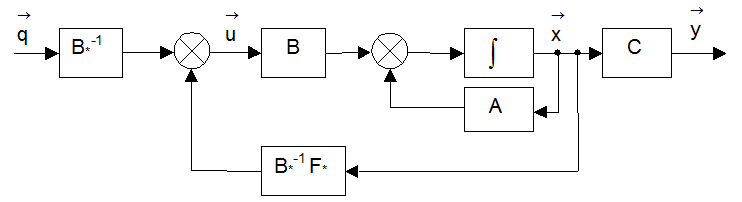
\includegraphics[scale=0.9]{images/Fig3_10}
	\caption{Промежуточная структурная схема}
\end{figure}
Для этой схемы справедливы уравнения
\begin{gather}
\begin{split}
	&\dot{\vec{x}}=(A+BB_*^{-1}F_*)\vec{x}+BB_*^{-1}\vec{q};\\
	&\vec{y}=C\vec{x}.
\end{split}
\end{gather}
Обозначим
\begin{gather}
\begin{split}
	&\underset{\lor}{A}=A+BB_*^{-1}F_*;\\
	&\underset{\lor}{B}=BB_*^{-1}.
\end{split}
\end{gather}
Теперь (3.10.11) превратится в 
\begin{equation}
\begin{cases}
	\dot{\vec{x}}=\underset{\lor}{A}\vec{x}+\underset{\lor}{B}\vec{q};\\
	\vec{y}=C\vec{x};
\end{cases}
\end{equation}
а структурная схема промежуточной системы с входным вектором $\vec{q}$ примет вид, представленный на рис. 3.11.
\begin{figure}[H]
	\centering
	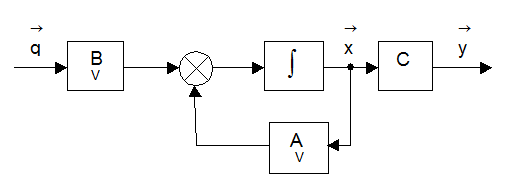
\includegraphics[scale=0.9]{images/Fig3_11}
	\caption{Структурная схема системы относительно входного вектора $\vec{q}$}
\end{figure}
С другой стороны, вектор выхода $\vec{y}$ связан с вектором $\vec{q}$ равенством (3.10.7), и поэтому схеме, представленной на рис. 3.11, полностью эквивалентна схема, составленная из $p$ подсистем последовательно включённых интеграторов. Эта схема представлена на рис. 3.12.
\begin{figure}[H]
	\centering
	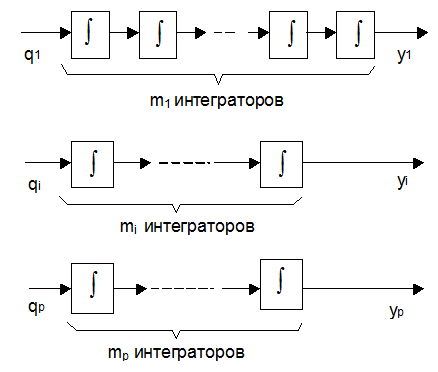
\includegraphics[scale=0.9]{images/Fig3_12}
	\caption{Структурная схема объекта, преставленного в виде изолированных подсистем интеграторов}
\end{figure}
Общее количество интеграторов не может быть больше $n$, то есть
\begin{equation*}
	\sum_{i=1}^{p}m_i\leq n.
\end{equation*}
Таким образом, система $\{\underset{\lor}{A},\underset{\lor}{B}\}$ (3.10.13), у которой в качестве входного вектора выбран вектор $\vec{q}$,

а) развязана по каналам, то есть $y_i$ зависит только от $q_i$ для всех значений $i$;

б) имеет $\sum_{i=1}^{p}m_i$ собственных значений, равных нулю.

Теперь систему $\{\underset{\lor}{A},\underset{\lor}{B}\}$ нужно попытаться привести к удобному базису, в котором следует синтезировать обратную связь, реализующую желаемые собственные числа по каждому каналу.

Прежде всего, установим некоторые свойства матриц $\underset{\lor}{A}$ и $\underset{\lor}{B}$. Аналогично (3.10.4) запишем:
\begin{equation*}
	y_i^{(m_i)}=C_i\underset{\lor}{A}^{m_i}\vec{x}+C_i\underset{\lor}{A}^{m_i-1}\underset{\lor}{B}\vec{q}+\sum_{v=1}^{m-1}C_i\underset{\lor}{A}^{m_i-1-v}\underset{\lor}{B}q^{(v)}.
\end{equation*}
С другой стороны, $y_i^{(m_i)}=q_i$. Отсюда следует:
\begin{equation}
	1) C_i\underset{\lor}{A}^{m_i}=0\text{ для всех }i=1,2,\dots,p;
\end{equation}
\begin{equation}
	2) C_i\underset{\lor}{A}^{m_i-1}\underset{\lor}{B}\vec{q}=C_i\underset{\lor}{A}^{m_i-1}
	\begin{bmatrix}
		 \underset{\lor}{\vec{b}_1} & \underset{\lor}{\vec{b}_2} & \dots & \underset{\lor}{\vec{b}_p}
	\end{bmatrix}\cdot
	\begin{bmatrix}
		 q_1\\q_1\\\vdots\\q_{ny}
	\end{bmatrix}=q_i,
\end{equation}
откуда
\begin{equation}
	C_i\underset{\lor}{A}^{m_i-1}\underset{\lor}{\vec{b}_i}=1;
\end{equation}
\begin{equation}
	C_i\underset{\lor}{A}^{m_i-1}\underset{\lor}{\vec{b}_j}=0,\text{ при } j\neq i;
\end{equation}
\begin{equation}
	3)C_i\underset{\lor}{A}^{m_i-v}\underset{\lor}{\vec{b}_j}=0,\text{ для } v>1 \text{ и для всех } j,i.
\end{equation}

\subsection{Преобразование базиса в пространстве $R^n$}
Перейдём от исходного базиса [$e$] к новому базису [$f$] с помощью некоторой матрицы преобразования $F_e$.  При выборе базиса [$f$] учтем следующие обстоятельства:
\begin{itemize}
\item объект управляем, поэтому ранг матрицы управляемости
\begin{equation}
	U=
	\setcounter{MaxMatrixCols}{20}
	\begin{bmatrix}
	\underset{\lor}{\vec{b}_1} & \underset{\lor}{\vec{b}_2} & \dots & \underset{\lor}{\vec{b}_p} & \vdots & \underset{\lor}{A}\underset{\lor}{\vec{b}_1} & \dots & \underset{\lor}{A}\underset{\lor}{\vec{b}_p} & \vdots & \dots & \vdots & \underset{\lor}{A^{n-1}}\underset{\lor}{\vec{b}_1} & \dots & \underset{\lor}{A^{n-1}}\underset{\lor}{\vec{b}_p}
	\end{bmatrix}
\end{equation} 
равен порядку системы;
\item так как каждый канал этой системы с размерностью $m_i$ управляем, то столбцы
\begin{equation*}
	\underset{\lor}{\vec{b}_1}, \underset{\lor}{A}\underset{\lor}{\vec{b}_1}, \dots, \underset{\lor}{A^{m_1-1}}\underset{\lor}{\vec{b}_1}, \dots, \underset{\lor}{\vec{b}_p}, \underset{\lor}{A}\underset{\lor}{\vec{b}_p}, \dots,
	\underset{\lor}{A^{m_p-1}}\underset{\lor}{\vec{b}_p}
\end{equation*}
линейно независимы.
\end{itemize}

Теперь выберем базис [$f$], соответствующий следующим координатным столбцам:
\begin{gather}
\begin{split}
	&\vec{f}_{e1}=\underset{\lor}{A^{m_1-1}}\underset{\lor}{\vec{b}_1}; \vec{f}_{e2}=\underset{\lor}{A^{m_1-2}}\underset{\lor}{\vec{b}_1};\dots; \vec{f}_{em_1}=\underset{\lor}{\vec{b}_1};\\
	&\vec{f}_{em_1+1}=\underset{\lor}{A^{m_2-1}}\underset{\lor}{\vec{b}_2}; \vec{f}_{em_1+2}=\underset{\lor}{A^{m_2-2}}\underset{\lor}{\vec{b}_2};\dots; \vec{f}_{em_1+m_2}=\underset{\lor}{\vec{b}_2};\\
	&\dots\dots\dots\dots\dots\dots\dots\dots\dots\\
	&\vec{f}_{em_1+\dots+m_{p-1}}=\underset{\lor}{A^{m_p-1}}\underset{\lor}{\vec{b}_p}; \vec{f}_{em_1+\dots+m_{p-2}}=\underset{\lor}{A^{m_p-2}}\underset{\lor}{\vec{b}_p}; \vec{f}_{em_1+\dots+m_p}=\underset{\lor}{\vec{b}_p}.
\end{split}
\end{gather}
Если $\sum_{i=1}^{p}m_i<n$, то оставшуюся часть векторов базиса [$f_{\text{ост}}$] можно выбирать, перебирая оставшиеся столбцы матрицы $U$:
\begin{equation*}
	\underset{\lor}{A^{m_1}}\underset{\lor}{\vec{b}_1},	\underset{\lor}{A^{m_1+1}}\underset{\lor}{\vec{b}_1},\dots	\underset{\lor}{A^{v_1-1}}\underset{\lor}{\vec{b}_1}
\end{equation*}
до тех пор, пока следующий вектор $	\underset{\lor}{A^v}\underset{\lor}{\vec{b}_1}$ не будет выражаться в виде линейной комбинации всех предыдущих векторов базиса. Далее добавим $\underset{\lor}{A^{m_2}}\underset{\lor}{\vec{b}_2},\underset{\lor}{A^{m_2+1}}\underset{\lor}{\vec{b}_2}$ и так далее, пока число векторов базиса не достигнет числа $n$. Тогда матрица преобразования базиса [$e$] в базис [$f$] будет иметь вид
\begin{equation*}
	F_e=
	\begin{bmatrix}
	\underset{\lor}{A^{m_1-1}}\underset{\lor}{\vec{b}_1} & \dots & \underset{\lor}{A^{m_1-2}}\underset{\lor}{\vec{b}_1} & \dots & \underset{\lor}{\vec{b}_1} & \dots & \underset{\lor}{A^{m_2-1}}\underset{\lor}{\vec{b}_2} & \dots & \underset{\lor}{\vec{b}_2} & \dots & \underset{\lor}{\vec{b}_p} & [f_\text{ост}]
	\end{bmatrix}
\end{equation*}

Рассмотрим вид матрицы $\underset{\lor}{B}$ в базисе [$f$]. Первый столбец этой матрицы, то есть вектор $\vec{b}_1$, совпадает с $m_1$-м столбцом базиса [$f$]; второй столбец матрицы $B$, то есть вектор $\vec{b}_2$, совпадает с $m_1+m_2$-м столбцом базиса [$f$] и так далее. Следовательно,
\begin{equation}
	B_e=
	\begin{bmatrix}
		\vec{\beta}_1 & 0 & \dots & 0\\
		0 & \vec{\beta}_2 & \dots & 0\\
		\dots & \dots & \dots & \dots\\
		0 & 0 & \dots & \vec{\beta}_p\\
		0 & 0 & \dots & 0
	\end{bmatrix},
\end{equation}
где
\begin{equation}
	\vec{\beta}_i=
	\begin{rcases}
	\begin{bmatrix}
		0\\0\\\dots\\0\\1
	\end{bmatrix}
	\end{rcases}m_i\text{ строк}
\end{equation}
Теперь обратим внимание на матрицу $C$. В соответствии с (3.6.8)
\begin{equation}
	C_f=CF_e=
	\begin{bmatrix}
		C_1\\C_2\\\vdots\\C_p
	\end{bmatrix}\cdot
	\begin{bmatrix}
		\vec{f}_{e_1} & \vec{f}_{e_2} & \dots & \vec{f}_{e_n}
	\end{bmatrix}=
	\begin{bmatrix}
		C_1\vec{f}_{e_1} & \dots & C_1\vec{f}_{e_n}\\
		C_2\vec{f}_{e_1} & \dots & C_2\vec{f}_{e_n}\\
		\dots & \dots & \dots\\
		C_p\vec{f}_{e_1} & \dots & C_p\vec{f}_{e_n}\\
	\end{bmatrix}
\end{equation}
Из этого равенства с учётом (3.10.14), (3.10.16), (3.10.17)  получим
\begin{equation}
	C_f=
	\begin{bmatrix}
		s_1 & 0 & \dots & 0 & 0\\
		0 & s_2 & \dots & 0 & 0\\
		\vdots & \vdots & \vdots & \vdots & \vdots\\
		0 & 0 & \dots & s_p & 0\\
	\end{bmatrix}
\end{equation}
где
\begin{equation}
	s_i=
	\underbrace{\begin{bmatrix}
		1 & 0 & \dots & 0
	\end{bmatrix}}_{m_i}.
\end{equation}

Наконец, займемся  матрицей $\underset{\lor}{A_f}$. Прежде всего, рассмотрим важную интерпретацию элементов матрицы $A_f$. В соответствии с (3.6.8)
\begin{equation*}
	A_f=F_e^{-1}A_eF_e,
\end{equation*}
поэтому
\begin{equation}
	F_eA_f=A_eF_e.
\end{equation}
Левую часть этого равенства можно расписать следующим образом:
\begin{gather*}
\begin{split}
	&F_eA_f=\begin{bmatrix}
	\vec{f}_{e1} & \vec{f}_{e2} & \dots & \vec{f}_{en}
	\end{bmatrix}\cdot
	\begin{bmatrix}
		a^f_{11} & a^f_{12} & \dots & a^f_{1n}\\
		\vdots & \vdots & \vdots & \vdots\\
		a^f_{n1} & a^f_{1n2} & \dots & a^f_{nn}\\
	\end{bmatrix}\\
	&=\begin{bmatrix}
		a^f_{11}\vec{f}_{e_1}+\dots+a^f_{n1}\vec{f}_{e_n} & a^f_{12}\vec{f}_{e_1}+\dots+a^f_{n2}\vec{f}_{e_n} & \dots & a^f_{1n}\vec{f}_{e_1}+\dots+a^f_{nn}\vec{f}_{e_n}
	\end{bmatrix}.
\end{split}
\end{gather*}
С другой стороны:
\begin{equation*}
	A_eF_e=[A_e\vec{f}_{e1}\dots A_e\vec{f_{e_n}}].
\end{equation*}
Таким образом, получаем
\begin{equation}
	A_e\vec{f}_{ei}=a^f_{1i}\vec{f}_{e1}+a^f_{2i}\vec{f}_{e2}+\dots+a^f_{ni}\vec{f}_{en}
\end{equation}
Это означает, что элементы $i$-го столбца матрицы $\underset{\lor}{A_f}$
\begin{equation*}
	\vec{a}_i^f=\begin{bmatrix}
	a^f_{1i}\\a^f_{2i}\\\dots\\a^f_{ni}
	\end{bmatrix}
\end{equation*}
являются коэффициентами разложения произведения $\underset{\lor}{A}\vec{f}_{ei}\equiv\underset{\lor}{A_e}\vec{f}_{ei}$ по координатным векторам $\vec{f}_{e1},\vec{f}_{e2},\dots,\vec{f}_{en}$.
Используя (3.10.20), сопоставим произведения ${A_e}\vec{f}_{ei}$ с координатными столбцами векторов базиса [$f$]:
\begin{gather}
\begin{split}
	&\underset{\lor}{A}\vec{f}_{e1}=\underset{\lor}{A^{m_1}}\underset{\lor}{\vec{b}_1};\\
	&\underset{\lor}{A}\vec{f}_{e2}=\underset{\lor}{A^{m_1-1}}\underset{\lor}{\vec{b}_1}=\vec{f}_{e1};\\
	&\underset{\lor}{A}\vec{f}_{e3}=\underset{\lor}{A^{m_1-2}}\underset{\lor}{\vec{b}_1}=\vec{f}_{e2};\\
	&\dots\dots\dots\dots\dots\dots
\end{split}
\end{gather}

Так как векторы $\underset{\lor}{A}f_{e1}$, $\underset{\lor}{A}f_{em_1+1}$ и т. д. не совпадают ни с одним из собственных векторов с номерами от 1 до $n-\sum_{i=1}^{p}m_i-1$, то в соответствующих столбцах матрицы $\underset{\lor}{A_f}$ на позициях строк с номерами, большими $p$, могут находиться ненулевые элементы. Такие ячейки матрицы помечены символом "$\times$". Кроме того, на данном этапе нет смысла рассматривать столбцы этой матрицы с номерами, большими $p$. В результате получаем выражение для матрицы $\underset{\lor}{A}$ в базисе [$f$]:	
\begin{figure}[H]
	\centering
	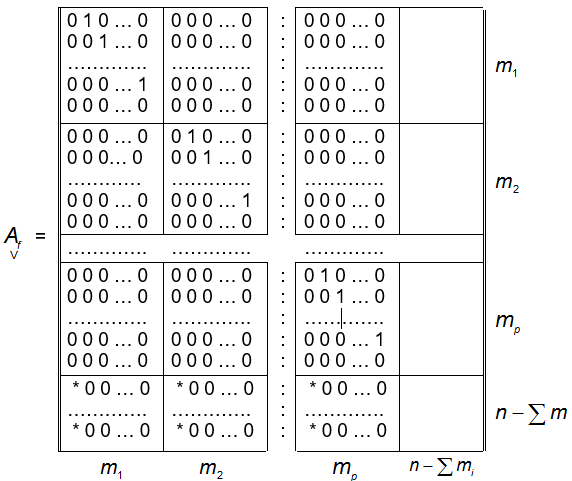
\includegraphics[scale=0.9]{images/Fig3_12_1}
\end{figure}
Эту же матрицу удобнее записать в блочном виде:
\begin{equation}
	\underset{\lor}{A}_f=\begin{bmatrix}
	A_{11} & 0 & \dots & 0 & A_{10}\\
	0 & A_{22} & \dots & 0 & A_{20}\\
	\vdots & \vdots & \vdots & \vdots & \vdots\\
	0 & 0 & \dots & A_{pp} & A_{p0}\\
	A_{01} & A_{02} & \dots & A_{0p} & A_{00}\\
	\end{bmatrix}.
\end{equation}

Разобьём вектор состояния $\vec{x}$ на систему $(p+1)$ частных векторов и обозначим
\begin{equation}
	\vec{x}_f=\begin{bmatrix}
	\vec{z}_1\\\vec{z}_2\\\vdots\vec{z}_p\\\vec{z}_0\\
	\end{bmatrix},
\end{equation}
где $\vec{z}_i$ имеет размерность [$m_i\times1$]. Тогда уравнения (3.10.13) в базисе [$f$] примут вид
\begin{equation*}
	\begin{bmatrix}
	\dot{\vec{z}}_1 \\ \dot{\vec{z}}_2 \\ \vdots \\ \dot{\vec{z}}_p \\ \dot{\vec{z}}_0
	\end{bmatrix}=
	\begin{bmatrix}
	A_{11} & 0 & \dots & 0 & A_{10}\\
	0 & a_{22} & \dots & 0 & A_{20}\\
	\vdots & \vdots & \vdots & \vdots & \vdots\\
	0 & 0 & \dots & A_{pp} & A_{p0}\\
	A_{01} & A_{02} & \dots & A_{0p} & A_{00}
	\end{bmatrix} * 
	\begin{bmatrix}
	\vec{z}_1 \\ \vec{z}_2 \\ \vdots \\ \vec{z}_p \\ \vec{z}_0   
	\end{bmatrix}+
	\begin{bmatrix}
	\vec{\beta}_1 & 0 & \dots & 0\\
	0 & \vec{\beta}_2 & \dots & 0\\
	\vdots & \vdots & \vdots & \vdots\\
	0 & 0 & \dots & \vec{\beta}_p\\
	0 & 0 & \dots & 0\\
	\end{bmatrix} * 
	\begin{bmatrix}
	q_1 \\ q_2 \\ \vdots \\ \vdots \\ q_p
	\end{bmatrix};
\end{equation*}
\begin{equation}
	\begin{bmatrix}
	y_1 \\ y_2 \\ \vdots \\ y_p
	\end{bmatrix}=
	\begin{bmatrix}
	s_1 & 0 & \dots & 0 & 0\\
	0 & s_2 & \dots & 0 & 0\\
	\vdots & \vdots & \vdots & \vdots & \vdots\\
	0 & 0 & \dots & s_p & 0
	\end{bmatrix}*
	\begin{bmatrix}
	\vec{z}_1 \\ \vec{z}_2 \\ \vdots \\ \vec{z}_p \\ \vec{z}_0   
	\end{bmatrix}
\end{equation}
Отсюда следуют уравнения для частных подсистем:
\begin{gather}
\begin{split}
	&\dot{\vec{z}}_i=A_{ii}\vec{z}_i+A_{i0}\vec{z}_0+\vec{\beta}_iq_i;\\
	&y_i=s_i\vec{z}_i, (i=1,2,\dots,p);
\end{split}
\end{gather}
\begin{equation}
\dot{\vec{z}}_0=\sum_{v=1}^{p}A_{0v}\vec{z}_v+A_{00}\vec{z}_0.
\end{equation}
Раскроем систему дифференциальных уравнений для $i$-й подсистемы:
\begin{equation}
\begin{cases}
\dot{z}_{i1}=z_{i2}+a_1^{i10}\vec{z}_0=z_{i2}+g{i1};\\
\dot{z}_{i2}=z_{i3}+g_{i2};\\
\dots\dots\dots\dots\dots\dots\\
\dot{z}_{i,m_i-1}=z_{i,m_i}+g_{i,m_i-1};\\
\dot{z}_{i,m_i}=g_{i,m_i}+q_i;
\end{cases}
\end{equation}
\begin{equation*}
\begin{cases}
y_i=z_{i1},
\end{cases}
\end{equation*}
где $a_1^{i10}$ - первая строка матрицы $A_{i0}$. Такой подсистеме соответствует структурная схема, представленная на рис. 3.13.
\begin{figure}[H]
	\centering
	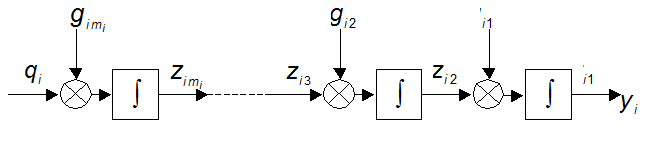
\includegraphics[scale=0.9]{images/Fig3_13}
	\caption{Структурная схема частотной подсистемы}
\end{figure}
Из сопоставления этой схемы со схемой, приведённой на рис. 3.12, следует:
a) $z_{i1}=y_i$; $z_{iv}=y_i^{(v)}$ при $v>1$;
б) $q_{iv}=0$ и $A_{v0}=0$ для $v=1,2,\dots,p$.

Таким образом,  выходы интеграторов частных подсистем, показанных на рис. 3.12, совпали с координатами вектора $\vec{x}$ в базисе [$f$].  Кроме того, все  блочные матрицы $A_{00},A_{10},\dots,A_{p0}$ в (3.10.29)- нулевые. 